% ----------------------------------------------------
\begin{frame}
  \titlepage
\end{frame}
% ----------------------------------------------------
\note{}

% ----------------------------------------------------
\begin{frame}
\frametitle{Today's second half}
\centering

\begin{itemize}[<+->]
\item The course has been about \textbf{estimation}: how to fit models
\item But fitting a model is rarely the hard part of empirical work
\item Today: what you actually need to answer a research question
  \begin{itemize}
  \item Research design and identification
  \item Causal inference methods beyond FE/DiD
  \item Defending your results: robustness and validity
  \item Common pitfalls when applying all of this
  \end{itemize}
\vspace{8pt}
\item Plus a pointer to two advanced topics (not covered today)
\end{itemize}

\end{frame}
% ----------------------------------------------------
\note{This lecture is deliberately different in tone from the rest of the course. We have spent the semester learning how to estimate a wide range of models. What I want to do today is to step back and make explicit the framing that sits behind all of that: what a regression actually gives you, what it does not, and what additional design choices make the difference between a credible empirical claim and a suggestive correlation. The goal is not to teach new techniques in the last hour of the course, but to give students a mental map they can carry into their final essay and into whatever they do next. The appendix at the end has pointers for two topics --- multilevel models and text as data --- that I will not cover in class but that students may want to explore on their own.}

% ====================================================
\section{From estimation to identification}
% ====================================================

% ----------------------------------------------------
\begin{frame}
\frametitle{What you have learned}
\centering

\begin{itemize}[<+->]
\item Estimation tools for many kinds of outcomes
  \begin{itemize}
  \item OLS, logit, count / ordinal / duration models
  \end{itemize}
\vspace{6pt}
\item Designs that exploit data structure
  \begin{itemize}
  \item Fixed effects, two-way FE, DiD (including staggered)
  \item Spatial models
  \end{itemize}
\vspace{6pt}
\item How to interpret and present results
  \begin{itemize}
  \item Predicted values, marginal effects, coefficient plots
  \end{itemize}
\vspace{6pt}
\item Plus computing practices to make all of this reproducible
\end{itemize}

\end{frame}
% ----------------------------------------------------
\note{Quick inventory of what the course has covered. The common thread is: given a research question and data, how do you go from raw numbers to a defensible estimate and a readable figure. That is real and useful work --- but it is only one piece of what empirical research actually requires. The next slides shift the frame.}

% ----------------------------------------------------
\begin{frame}
\frametitle{Two different questions}
\centering

\vspace{15pt}

\begin{itemize}
\item[] \textbf{Estimation:} given a model, what are the parameters?
\vspace{15pt}
\item[] \textbf{Identification:} do those parameters mean what I think they mean?
\end{itemize}

\vspace{25pt}

\only<2->{\centering Your R output answers the first.\\ \vspace{6pt} Only your research design can answer the second.}

\end{frame}
% ----------------------------------------------------
\note{This is the central distinction. Estimation is a statistical problem: given a specification, compute the best-fit coefficients. R will always give you a number. Identification is a research-design problem: does the coefficient you just estimated correspond to the causal (or descriptive) quantity you actually want to learn about? The reason identification is hard is that the same regression output is consistent with many different underlying data-generating processes, and you cannot tell them apart from the estimation alone. You need theory and design assumptions.}

% ----------------------------------------------------
\begin{frame}
\frametitle{The fundamental problem of causal inference}
\centering

\begin{itemize}[<+->]
\item A \textbf{causal effect} is the difference between what \textit{did} happen and what \textit{would have} happened otherwise
\vspace{6pt}
\item For unit $i$ with treatment $D$:
  \[
    \tau_i = Y_i(1) - Y_i(0)
  \]
\vspace{-6pt}
\item We only ever observe \textbf{one} of these two worlds
  \begin{itemize}
  \item If $i$ was treated, $Y_i(1)$ is observed and $Y_i(0)$ is missing
  \item If $i$ was not treated, the opposite
  \end{itemize}
\vspace{6pt}
\item Causal inference $=$ principled way to estimate the missing counterfactual
\end{itemize}

\end{frame}
% ----------------------------------------------------
\note{The potential outcomes framework in one slide. Emphasize that this is a missing data problem in disguise: for any given unit, half of the information we would need to compute a causal effect is unobservable. Everything else --- randomization, fixed effects, DiD, IV, RDD, matching --- is machinery for building a credible estimate of that missing counterfactual. If the counterfactual is not credible, the machinery does not help.}

% ----------------------------------------------------
\begin{frame}
\frametitle{What we can estimate on average}
\centering

\begin{itemize}
\item We can't recover $\tau_i$ for individuals
\vspace{8pt}
\item But we can target averages:
  \begin{itemize}
  \item \textbf{ATE} --- average over everyone: $E[Y(1) - Y(0)]$
  \item \textbf{ATT} --- average over the treated: $E[Y(1) - Y(0)\,|\,D=1]$
  \item \textbf{LATE} --- average over those who \textit{respond} to a treatment (IV, RDD)
  \end{itemize}
\vspace{8pt}
\item Different methods estimate different quantities
  \begin{itemize}
  \item When you compare two papers: are they even targeting the same thing?
  \end{itemize}
\end{itemize}

\end{frame}
% ----------------------------------------------------
\note{A useful sanity-check when reading applied papers: which of these averages is the estimator targeting? A randomized experiment gives you the ATE over the experimental sample. A DiD gives you the ATT on the treated units. An IV or RDD gives you a LATE, a local effect for those whose treatment status is actually driven by the instrument or the cutoff. These are different quantities. Two papers can report conflicting effects on the same phenomenon simply because they are estimating different averages over different subpopulations.}

% ----------------------------------------------------
\begin{frame}
\frametitle{Causal models and DAGs}
\centering

\begin{itemize}[<+->]
\item To approximate the counterfactual we need a model of \textit{why} units are treated in the first place
\vspace{6pt}
\item Directed Acyclic Graphs (DAGs): nodes are variables, arrows are direct causal effects
\vspace{6pt}
\item Three structures you must recognize:
  \begin{itemize}
  \item \textbf{Confounder} \quad $D \leftarrow Z \rightarrow Y$
  \item \textbf{Mediator} \quad $D \rightarrow M \rightarrow Y$
  \item \textbf{Collider} \quad $D \rightarrow C \leftarrow Y$
  \end{itemize}
\vspace{6pt}
\item What you control for --- and what you do \textbf{not} --- depends on which structure you are looking at
\end{itemize}

\end{frame}
% ----------------------------------------------------
\note{DAGs are the most compact way to talk about what a regression is really doing when you add a control variable. The three structures on this slide cover most of the cases you will see. The non-obvious rule: you want to control for confounders, you should not control for mediators (that blocks the effect you are trying to measure), and you should absolutely not control for colliders (that opens a spurious path).}

% ----------------------------------------------------
\begin{frame}
\frametitle{Confounding: the standard case}
\centering

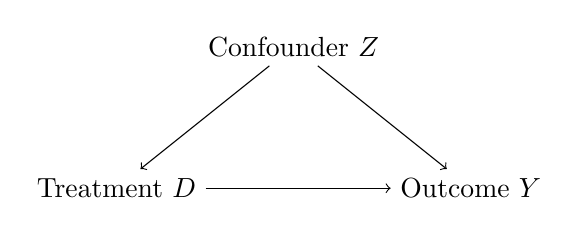
\begin{tikzpicture}[every node/.style={align=center}, scale=0.9]
  \node (D) at (0,0){Treatment $D$};
  \node (Y) at (5,0){Outcome $Y$};
  \node (Z) at (2.5,2){Confounder $Z$};
  \draw[->] (D) -- (Y);
  \draw[->] (Z) -- (D);
  \draw[->] (Z) -- (Y);
\end{tikzpicture}

\vspace{15pt}

\begin{itemize}
\item $Z$ affects both $D$ and $Y$: a \BGyellow{back-door path}
\item Un-adjusted comparison of treated vs.\ untreated mixes two effects
\item \textbf{Solution:} condition on $Z$ (or use a design that blocks the back door)
\end{itemize}

\end{frame}
% ----------------------------------------------------
\note{Ice-cream sales and drownings; pirate numbers and global temperature. These are the textbook examples, but confounding is also the implicit story behind every ``we add controls for $X$, $Y$, $Z$'' paragraph in an empirical paper. Every control you add should correspond to a node on a DAG that your theory justifies. Adding controls because they change the coefficient is how you generate p-hacked results.}

% ----------------------------------------------------
\begin{frame}
\frametitle{Colliders: do not control!}
\centering

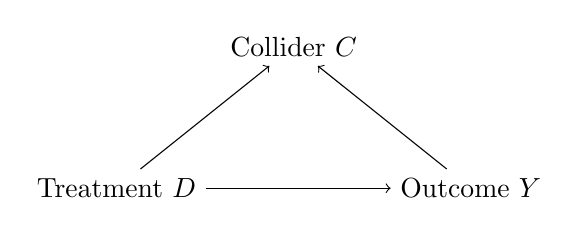
\begin{tikzpicture}[every node/.style={align=center}, scale=0.9]
  \node (D) at (0,0){Treatment $D$};
  \node (Y) at (5,0){Outcome $Y$};
  \node (C) at (2.5,2){Collider $C$};
  \draw[->] (D) -- (Y);
  \draw[->] (D) -- (C);
  \draw[->] (Y) -- (C);
\end{tikzpicture}

\vspace{15pt}

\begin{itemize}
\item $C$ is caused \textit{by} both $D$ and $Y$
\item Conditioning on $C$ creates a spurious association between $D$ and $Y$
\item Classic: ``smart people lack social skills'' (if you condition on being hired)
\end{itemize}

\end{frame}
% ----------------------------------------------------
\note{The counterintuitive result in causal inference: some variables make the bias worse when you add them as controls. A collider is any variable that is downstream of both your treatment and your outcome. Conditioning on it opens a non-causal path between the two. The standard illustration: intelligence and social skills may be uncorrelated in the population, but if you restrict attention to people hired at a competitive company (which selects on both), you will find a spurious negative correlation.}

% ----------------------------------------------------
\begin{frame}
\frametitle{Post-treatment bias}
\centering

\begin{itemize}[<+->]
\item Special case of collider bias that is very easy to miss
\item A \textbf{post-treatment} variable is one that is itself affected by the treatment
\item Controlling for it:
  \begin{itemize}
  \item blocks part of the mechanism (if it is a mediator), \textbf{or}
  \item opens a collider path (if it is also affected by other unobservables)
  \end{itemize}
\vspace{6pt}
\item Rule of thumb: if in doubt about whether a variable is pre- or post-treatment, leave it out
\end{itemize}

\end{frame}
% ----------------------------------------------------
\note{Post-treatment bias is the single most common avoidable mistake in applied work. Typical pattern: researcher estimates the effect of a treatment, worries that results might be confounded, throws in every variable available including some that were measured after the treatment. Those post-treatment variables either sit on the causal pathway the researcher is trying to measure (so controlling for them attenuates the effect mechanically) or open collider paths (so controlling for them introduces bias). Montgomery, Nyhan and Torres 2018 AJPS is the reference; keep it in mind when you are writing your final essay.}

% ----------------------------------------------------
\begin{frame}
\frametitle{Post-treatment bias: example}
\centering

\vspace{5pt}

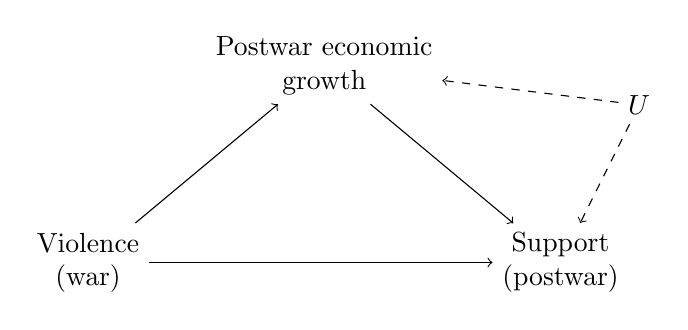
\begin{tikzpicture}[every node/.style={align=center}]
  \node (D) at (-2.5,0){Violence\\(war)};
  \node (Y) at (3.5,0){Support\\(postwar)};
  \node (Z) at (0.5,2.5){Postwar economic\\growth};
  \node (U) at (4.5,2){$U$};
  \draw[->] (D) -- (Y);
  \draw[<-] (Z) -- (D);
  \draw[->] (Z) -- (Y);
  \draw[->, dashed] (U) -- (Z);
  \draw[->, dashed] (U) -- (Y);
\end{tikzpicture}

\vspace{10pt}

\begin{itemize}
\item Does wartime violence affect postwar political support?
\item ``Let's control for postwar economic growth, it also affects support''
\item But growth is \textbf{caused by} the treatment \textit{and} shares unobservables with the outcome --- controlling for it opens a back door
\end{itemize}

\end{frame}
% ----------------------------------------------------
\note{A concrete example of post-treatment bias. Suppose the question is whether experiencing wartime violence changes people's postwar political attitudes. A reasonable-sounding move would be to control for postwar economic growth, since growth also affects political support. The DAG shows why this is wrong: growth is a \textit{consequence} of the wartime violence (treated areas develop differently after the war), and growth and support share unobserved causes $U$. Conditioning on growth therefore opens a collider path from violence to support through $U$, introducing exactly the bias the researcher was trying to avoid. The rule is not \"control for everything that affects $Y$\"; it is \"control for pre-treatment confounders only\".}

% ----------------------------------------------------
\begin{frame}
\frametitle{So what does your regression assume?}
\centering

\vspace{20pt}

Every regression coefficient you report implicitly assumes:

\vspace{10pt}

\begin{itemize}
\item[1.] You have \textbf{closed all back doors} (no omitted confounders)
\vspace{4pt}
\item[2.] You have \textbf{not opened new ones} (no controlling for colliders or mediators)
\vspace{4pt}
\item[3.] The functional form is roughly right (linearity, additivity)
\end{itemize}

\vspace{15pt}

\only<2->{\centering (1) and (2) are \textbf{design} assumptions, not something you can test.}

\end{frame}
% ----------------------------------------------------
\note{Wrap up the first section. The assumptions that matter most are the ones that cannot be checked from the data alone --- they come from your theory and your argument about the data-generating process. This is why a paper's identification strategy is more important than its R-squared.}

% ====================================================
\section{Causal inference toolkit}
% ====================================================

% ----------------------------------------------------
\begin{frame}
\frametitle{What you already have}
\centering

\begin{itemize}
\item[] Two of the four big causal-inference designs are already in your toolkit:
\vspace{10pt}
\item \textbf{Fixed effects} --- control for all time-invariant unobservables at some level (unit, region, year\ldots)
\vspace{6pt}
\item \textbf{Difference-in-differences} --- use a never-treated comparison group plus pre/post variation; identifies the ATT under parallel trends
\vspace{10pt}
\item[] Two more that you should at least recognize:
\vspace{6pt}
\item \textbf{Regression discontinuity design (RDD)}
\item \textbf{Instrumental variables (IV)}
\end{itemize}

\end{frame}
% ----------------------------------------------------
\note{Recap what we have, flag what we still need to cover at a high level. I do not expect students to leave this lecture able to run an RDD or an IV regression --- I want them to recognize these designs when they encounter them, understand the intuition, and know when a problem calls for them.}

% ----------------------------------------------------
\begin{frame}
\frametitle{Estimating DiD}
\centering

\begin{itemize}[<+->]
\item DiD is not a special estimator --- it's just OLS on a 2$\times$2 interaction
\vspace{4pt}
\item[] \quad $Y_{it} = \alpha + \beta_1 \text{Treat}_i + \beta_2 \text{Post}_t + \beta_3 (\text{Treat}_i \times \text{Post}_t) + \varepsilon_{it}$
\vspace{4pt}
\item \BGyellow{$\beta_3$} is the DiD estimate
\vspace{8pt}
\item In practice: two-way fixed effects absorb $\text{Treat}_i$ and $\text{Post}_t$
\item[] \quad \texttt{feols(y \textasciitilde{} treat\_post | unit + time, data = d)}
\vspace{8pt}
\item For staggered adoption: use modern estimators (Callaway--Sant'Anna, Sun--Abraham) --- see Session 6
\end{itemize}

\end{frame}
% ----------------------------------------------------
\note{Bring the DiD estimation back to earth: it is not a new statistical method, it is OLS with an interaction term. The interaction coefficient is the DiD. Two-way fixed effects is the scalable way to do this when you have many units and many time periods: the unit FEs absorb the treatment-group indicator, the time FEs absorb the post indicator, and you are left with the interaction as your coefficient of interest. The only complication is staggered adoption, which breaks classic TWFE --- that's what the Callaway--Sant'Anna and Sun--Abraham estimators fix, and we covered them in Session 6.}

% ----------------------------------------------------
\begin{frame}
\frametitle{Regression discontinuity design}
\centering

\begin{itemize}[<+->]
\item \textbf{Setup:} treatment assignment depends on whether a \textit{running variable} crosses a cutoff
  \begin{itemize}
  \item Incumbency advantage: winners of close elections
  \item Scholarships: eligibility based on test score cutoff
  \item Conscription: draft lottery numbers below a threshold
  \end{itemize}
\vspace{6pt}
\item \textbf{Idea:} units just above and just below the cutoff should be similar in everything \textit{except} the treatment
\vspace{6pt}
\item Estimates a \BGyellow{LATE}: effect for units near the threshold
\end{itemize}

\end{frame}
% ----------------------------------------------------
\note{RDD has become one of the most popular designs in political science over the last decade, largely because close-election data is readily available and the identification assumption is transparent. Important caveat students should know: an RDD estimate only tells you about units near the cutoff. The effect of a scholarship for marginal admits may look very different from the effect for a student who was a clear admit.}

% ----------------------------------------------------
\begin{frame}
\frametitle{RDD visually}
\centering

\vspace{10pt}

\begin{tikzpicture}[scale=0.7]
  % axes
  \draw[->] (0,0) -- (10,0) node[right]{Running variable};
  \draw[->] (0,0) -- (0,6) node[above]{$Y$};
  % cutoff
  \draw[dashed] (5,0) -- (5,5.5);
  \node[below] at (5,0){cutoff};
  % left trend
  \draw[thick, accent] (0.5,1) -- (5,3);
  % right trend (with jump)
  \draw[thick, accent2] (5,4.5) -- (9.5,5.5);
  % jump indicator
  \draw[<->, thick] (5.1,3) -- (5.1,4.5);
  \node[right] at (5.15,3.75){\small effect};
\end{tikzpicture}

\vspace{10pt}

\begin{itemize}
\item The jump at the cutoff is the treatment effect
\item The trend on each side controls for whatever else varies smoothly
\end{itemize}

\end{frame}
% ----------------------------------------------------
\note{This picture is the whole argument. We believe any confounders vary smoothly as the running variable moves. At the cutoff, treatment changes discretely while everything else stays continuous. So a discontinuity in the outcome at that point can only be caused by the treatment. The design can fail if people can precisely manipulate their position around the cutoff, or if the cutoff triggers other changes besides the treatment of interest.}

% ----------------------------------------------------
\begin{frame}
\frametitle{Estimating RDD}
\centering

\begin{itemize}[<+->]
\item Center the running variable at the cutoff: $\tilde{X}_i = X_i - c$
\item Define treatment: $D_i = \mathbf{1}(\tilde{X}_i \geq 0)$
\vspace{6pt}
\item Run a local linear regression with slopes allowed to differ on each side:
\item[] \quad $Y_i = \alpha + \tau D_i + \beta_1 \tilde{X}_i + \beta_2 (D_i \times \tilde{X}_i) + \varepsilon_i$
\vspace{4pt}
\item $\tau$ is the RDD estimate (the jump at the cutoff)
\vspace{8pt}
\item Key choice: \BGyellow{bandwidth} --- how wide a window around the cutoff
  \begin{itemize}
  \item Data-driven: Calonico, Cattaneo \& Titiunik
  \end{itemize}
\vspace{4pt}
\item R: \texttt{rdrobust::rdrobust(y, x, c = 0)}
  \begin{itemize}
  \item \texttt{c} is the cutoff value of the running variable \texttt{x}
  \end{itemize}
\end{itemize}

\end{frame}
% ----------------------------------------------------
\note{RDD estimation in practice. The conceptual version is: fit a line on each side of the cutoff, report the gap between them at the cutoff. That is what the interacted specification does --- one intercept and slope for units below the cutoff, a different intercept and slope for units above, and the discontinuity $\tau$ is the difference in intercepts at $\tilde{X} = 0$. The one real choice is the bandwidth: how far from the cutoff do you include observations? Wider windows give more data but risk bias from units far from the threshold; narrower windows are less biased but noisier. The \\texttt{rdrobust} package implements the Calonico-Cattaneo-Titiunik data-driven bandwidth selector, which is the current default in applied work. The \\texttt{c} argument is the cutoff value of the running variable: set \\texttt{c = 0} when you have already centered \\texttt{x} at the threshold, otherwise pass the actual cutoff (for example \\texttt{c = 50} for a vote-share majority rule).}

% ----------------------------------------------------
\begin{frame}
\frametitle{Instrumental variables}
\centering

\begin{tikzpicture}[every node/.style={align=center}, scale=0.9]
  \node (Z) at (-1,0){Instrument $Z$};
  \node (D) at (4,0){Treatment $D$};
  \node (Y) at (8,0){Outcome $Y$};
  \node (U) at (6,2){$U$};
  \draw[->] (Z) -- (D);
  \draw[->] (D) -- (Y);
  \draw[->, dashed] (U) -- (D);
  \draw[->, dashed] (U) -- (Y);
\end{tikzpicture}

\vspace{15pt}

\begin{itemize}[<+->]
\item Find a variable $Z$ that moves $D$ but has no other path to $Y$
\item Use only the variation in $D$ explained by $Z$
\item Two assumptions:
  \begin{itemize}
  \item \textbf{Relevance}: $Z$ actually affects $D$ (testable)
  \item \textbf{Exclusion restriction}: $Z$ affects $Y$ only through $D$ (not testable)
  \end{itemize}
\end{itemize}

\end{frame}
% ----------------------------------------------------
\note{The IV design. Classic examples: rainfall as an instrument for protest intensity (rainfall shifts who shows up to a protest, but should not affect whatever political outcome you are studying except through its effect on protests). The canonical problem with IV in practice is the exclusion restriction: you have to tell a story about why the instrument could not plausibly affect the outcome by any route other than through the treatment. That story is often contested.}

% ----------------------------------------------------
\begin{frame}
\frametitle{Estimating IV: two-stage least squares}
\centering

\begin{itemize}[<+->]
\item \textbf{First stage:} regress the treatment on the instrument
\item[] \quad $D_i = \pi_0 + \pi_1 Z_i + u_i \;\; \Rightarrow \;\; \hat{D}_i$
\vspace{4pt}
\item \textbf{Second stage:} regress the outcome on the \textit{predicted} treatment
\item[] \quad $Y_i = \alpha + \beta \hat{D}_i + \varepsilon_i$
\vspace{6pt}
\item \BGyellow{$\beta$} is the IV estimate: a LATE for units whose $D$ responds to $Z$
\vspace{10pt}
\item Always report the first stage, and an \BGyellow{F-statistic} on $\pi_1$
  \begin{itemize}
  \item Rule of thumb: $F < 10$ signals a weak instrument
  \end{itemize}
\vspace{4pt}
\item R: \texttt{feols(y \textasciitilde{} 1 | d \textasciitilde{} z)} or \texttt{AER::ivreg()}
\end{itemize}

\end{frame}
% ----------------------------------------------------
\note{The mechanics of 2SLS. Conceptually: first project the treatment onto the instrument, keeping only the variation in $D$ that is driven by $Z$. Then use that projected treatment in the outcome equation. The second-stage coefficient is the IV estimate. Two things to emphasize. First, what you estimate is a LATE, not the ATE: it is the effect for the \\textit{compliers}, the units whose treatment status actually responds to the instrument. That is often a subset of the population and may not be who you care about. Second, always show the first stage. A weak first stage --- conventionally an F-statistic below 10 on the instrument --- means your 2SLS estimates can be badly biased and have completely unreliable standard errors. Do not skip this diagnostic.}

% ----------------------------------------------------
\begin{frame}
\frametitle{The four design templates}
\centering

\vspace{10pt}

\renewcommand{\arraystretch}{1.3}
\footnotesize
\begin{tabular}{p{1.6cm}p{3.5cm}p{4cm}}
\hline
\textbf{Design} & \textbf{Exogenous variation} & \textbf{Key assumption}\\
\hline
FE & Within-unit differences & No time-varying confounders\\
DiD & Treated vs.\ comparison, pre/post & Parallel trends\\
RDD & Jump at cutoff & No manipulation at cutoff\\
IV & Instrument $\rightarrow$ treatment & Exclusion restriction\\
\hline
\end{tabular}

\vspace{12pt}

\begin{itemize}
\item \footnotesize You do not pick a design, \textit{the data} pick one for you
\item \footnotesize What source of exogenous variation does the world hand you?
\end{itemize}

\end{frame}
% ----------------------------------------------------
\note{The design-based approach to causal inference, in one slide. A good applied paper starts from a research question and a dataset and asks: what source of variation in this setting can I credibly treat as exogenous? The answer to that question determines the method. It is very rarely the case that the researcher picks the method first and then looks for a matching application.}

% ----------------------------------------------------
\begin{frame}
\frametitle{Matching: complement, not substitute}
\centering

\begin{itemize}[<+->]
\item Not a design in the same sense --- but a useful preprocessing step
\item \textbf{Idea:} pair each treated unit with one or more untreated units that look similar on observed covariates
\item Compare only within matched pairs
\vspace{6pt}
\item What it fixes: imbalance in observed covariates and reliance on linear-in-parameters extrapolation
\item What it does \textbf{not} fix: omitted confounders, selection on unobservables
\vspace{6pt}
\item Often used \textit{with} regression or DiD, not instead of
\end{itemize}

\end{frame}
% ----------------------------------------------------
\note{Matching is sometimes presented as a rival to regression; it is better understood as a complement. Both methods deal with the same problem --- conditioning on observed covariates --- but matching makes the comparisons more transparent and less dependent on functional-form assumptions. If the two agree, you are on firmer ground. If they disagree, something about your specification is doing a lot of the work.}

% ====================================================
\section{Defending a causal claim}
% ====================================================

% ----------------------------------------------------
\begin{frame}
\frametitle{Your main result is the beginning}
\centering

\vspace{20pt}

\begin{itemize}
\item You have a point estimate, a standard error, a figure
\vspace{8pt}
\item A skeptical reader should be asking:
  \begin{itemize}
  \item What if you had specified it differently?
  \item What if your identifying assumption is wrong?
  \item What if you are measuring the wrong thing?
  \item Would the result generalize elsewhere?
  \end{itemize}
\vspace{10pt}
\item Your job is to answer those questions \textbf{before they do}
\end{itemize}

\end{frame}
% ----------------------------------------------------
\note{Framing for the third section. A published empirical paper is not just the main result; it is the main result plus a set of complementary analyses that demonstrate the result is not an artifact of specification, assumption, measurement, or sample. If students take one piece of practical advice from this lecture, it should be: plan those complementary analyses before you run the main model, not afterwards as damage control.}

% ----------------------------------------------------
\begin{frame}
\frametitle{Robustness: alternative specifications}
\centering

\begin{itemize}[<+->]
\item Change one thing at a time, show it does not matter much
\vspace{6pt}
\item Measurement of $Y$: alternative indicators, different scales
\item Measurement of $D$: dichotomize vs.\ continuous, source
\item Sample: drop influential units, drop specific sub-groups
\item Model: add/remove controls, change FE structure, change SEs
\item Functional form: log, quadratic, non-parametric
\vspace{6pt}
\item Display as a \BGyellow{coefficient plot across specifications}, not a 10-column table no one reads
\end{itemize}

\end{frame}
% ----------------------------------------------------
\note{When you change a measurement choice or a modeling choice, the coefficient should move, but the substantive story should not. The goal is not to show that the point estimate is identical across specifications (it won't be); it is to show that the \\textit{conclusion} is robust. The visualization matters --- a specification curve or a coefficient plot across many specifications is much more convincing than a kitchen-sink regression table.}

% ----------------------------------------------------
\begin{frame}
\frametitle{Placebo tests}
\centering

\begin{itemize}[<+->]
\item Look for an effect \textit{where there should be none}
\vspace{6pt}
\item If you find it, something is wrong with your design
\vspace{10pt}
\item Three flavors (Eggers, Tu\~n\'on \& Dafoe 2023):
  \begin{itemize}
  \item \textbf{Placebo outcome}: different $Y$ that the treatment should not affect
  \item \textbf{Placebo treatment}: a fake $D$ that should have no effect
  \item \textbf{Placebo population}: a subgroup not exposed to $D$
  \end{itemize}
\vspace{6pt}
\item Example --- Peisakhin \& Rozenas (2018), Russian TV in Ukraine:
  \begin{itemize}
  \item[$\circ$] Outcome: signal strength should not predict \% Russian speakers
  \item[$\circ$] Treatment: Russian \textit{sports} TV signal should not predict voting
  \item[$\circ$] Population: Ukrainians on satellite TV --- signal irrelevant
  \end{itemize}
\end{itemize}

\end{frame}
% ----------------------------------------------------
\note{Placebos are the most intuitive tool for checking an identification assumption. If you claim that your effect is driven by a specific mechanism, there should be outcomes, treatments, or populations where that mechanism cannot plausibly operate. If you find the same-sized effect there too, that is evidence your identification is picking up something other than what you think. A classic example is the Peisakhin \& Rozenas study on Russian TV: they show that sports-channel signal strength does not predict voting, which builds confidence that the news-channel result is about content and not about something generic like TV reception quality.}

% ----------------------------------------------------
\begin{frame}
\frametitle{Placebo tests in DiD}
\centering

\begin{itemize}[<+->]
\item Most important placebo in a DiD setup: \textbf{pre-trends}
\item Before the treatment, the two groups should move in parallel
\item If pre-treatment "leads" are significant, parallel trends is suspect
\vspace{10pt}
\item Event-study plots show this visually:
  \begin{itemize}
  \item Coefficients on event-time dummies
  \item Pre-period coefficients should be flat and near zero
  \item Post-period coefficients show the dynamic effect
  \end{itemize}
\end{itemize}

\end{frame}
% ----------------------------------------------------
\note{This ties back to Session 6. Event-study plots are the workhorse visualization for modern DiD work. The pre-treatment portion is itself a placebo test: if the treatment has not happened yet, there should be no treatment effect. A slope in the pre-period is evidence that your comparison group was not a good counterfactual to begin with.}

% ----------------------------------------------------
\begin{frame}
\frametitle{Additional implications}
\centering

\begin{itemize}[<+->]
\item If your theory is correct, what \textit{else} should be true in the data?
\vspace{6pt}
\item \textbf{Mechanism checks}: intermediate variables your theory predicts
\item \textbf{Heterogeneity}: groups where the effect should be larger or smaller
\item \textbf{Rule-out tests}: observable patterns that competing explanations would imply but yours would not
\vspace{8pt}
\item A paper that only shows the main effect is weaker than one that shows the main effect \textbf{plus} two or three such auxiliary findings
\end{itemize}

\end{frame}
% ----------------------------------------------------
\note{Strong empirical papers do not just test their main hypothesis; they derive and test auxiliary implications of their theory. This is where the research-design framing pays off: a well-specified theory will imply patterns of heterogeneity (the effect should be larger among group X), mechanism predictions (intermediate variable M should move with the treatment), and exclusion patterns (if the competing explanation were right, we would see Y, but we see Z instead). This is what turns an empirical paper from ``I ran a regression'' into ``I used the data to discriminate between competing accounts.''}

% ----------------------------------------------------
\begin{frame}
\frametitle{Measurement and construct validity}
\centering

\begin{itemize}[<+->]
\item Are you measuring what you think you are measuring?
\vspace{6pt}
\item \textbf{Treatment}: when you say $D = 1$, what is actually being delivered?
  \begin{itemize}
  \item Bundled treatments (media exposure $=$ content $+$ format $+$ novelty$\ldots$)
  \end{itemize}
\vspace{6pt}
\item \textbf{Outcome}: does the indicator really capture the concept?
  \begin{itemize}
  \item Polarization $=$ partisan thermometer gap? policy-view distance? affective feelings?
  \end{itemize}
\vspace{8pt}
\item Identification can be perfect and the claim still be wrong if the measurement doesn't line up with the theory
\end{itemize}

\end{frame}
% ----------------------------------------------------
\note{Measurement is underrated. A perfectly identified estimate of something that is not what you wanted to measure is not progress. Ask, for any paper you read: what would have to be true for the reported indicator to really capture the concept the author talks about in the introduction? Often the answer is ``a lot'' and that creates space for disagreement even when the design is clean.}

% ----------------------------------------------------
\begin{frame}
\frametitle{External validity}
\centering

\begin{itemize}[<+->]
\item Under what \textit{conditions} does the effect hold?
\item Four dimensions (Egami \& Hartman 2023):
  \begin{itemize}
  \item \textbf{Populations}: units beyond your sample
  \item \textbf{Treatments}: variants of the intervention
  \item \textbf{Outcomes}: related but different $Y$s
  \item \textbf{Contexts}: other settings, places, times
  \end{itemize}
\vspace{8pt}
\item A clean estimate in one sample does not automatically generalize
\item \textbf{Temporal validity} (Munger 2023): does it still hold 10 years from now?
\end{itemize}

\end{frame}
% ----------------------------------------------------
\note{External validity is the question most often brushed aside with a single paragraph in the conclusion. Egami and Hartman offer a usable framework: rather than treating external validity as a yes/no question, decompose it into specific dimensions and ask which ones plausibly transfer and which do not. The temporal dimension is particularly salient in fast-moving domains like social media research, where the platform you studied five years ago may not exist in the same form today.}

% ====================================================
\section{Choosing the right method \& pitfalls}
% ====================================================

% ----------------------------------------------------
\begin{frame}
\frametitle{Starting point: your question type}
\centering

\renewcommand{\arraystretch}{1.4}
\footnotesize
\begin{tabular}{p{3.3cm}p{7cm}}
\hline
\textbf{Goal} & \textbf{Tools}\\
\hline
Describe a pattern & Summary stats, visualization, simple regression\\
Predict $Y$ from $X$ & Regression, ML (cross-validated)\\
Explain $Y$ causally & Design-based methods: FE, DiD, RDD, IV, experiments\\
Generalize a mechanism & Theory + replication across contexts\\
\hline
\end{tabular}

\vspace{15pt}

\begin{itemize}
\item Most confusion in applied work comes from mixing these up
  \begin{itemize}
  \item e.g.\ treating predictive coefficients as causal
  \end{itemize}
\end{itemize}

\end{frame}
% ----------------------------------------------------
\note{If you take one thing from this slide: be explicit about what kind of question you are trying to answer, because the standards of evidence differ. A predictive model can be judged on out-of-sample performance and does not need causal identification. A causal claim needs an identification strategy and out-of-sample performance is secondary. A descriptive paper needs neither but requires careful measurement and framing. Papers that slide between these modes are weaker than papers that commit to one.}

% ----------------------------------------------------
\begin{frame}
\frametitle{Starting point: your outcome}
\centering

\renewcommand{\arraystretch}{1.4}
\footnotesize
\begin{tabular}{p{3.5cm}p{6cm}}
\hline
\textbf{Outcome type} & \textbf{Method}\\
\hline
Continuous & OLS (always a good first pass)\\
Binary & Logit, probit (or LPM for interpretability)\\
Count (non-negative integer) & Poisson, negative binomial\\
Ordered categories & Ordered logit / probit\\
Time-to-event & Cox, Kaplan–Meier, parametric survival\\
Panel data & + fixed effects, + clustered SEs\\
Spatial data & + spatial weights, + Moran's I\\
\hline
\end{tabular}

\vspace{10pt}

\begin{itemize}
\item \footnotesize This is a cheat-sheet for your final essay --- keep it
\end{itemize}

\end{frame}
% ----------------------------------------------------
\note{The cheat-sheet version of the whole course. This is not a substitute for understanding what each model does; it is a decision aid for when you are staring at a dataset and trying to pick a starting point. For most social science questions, the answer is ``OLS first, then something more specialized if the defaults are clearly wrong.''}

% ----------------------------------------------------
\begin{frame}
\frametitle{Pitfall 1: p-hacking and forking paths}
\centering

\begin{itemize}[<+->]
\item Garden of forking paths (Gelman \& Loken 2013)
\vspace{6pt}
\item Every analysis involves many small choices:
  \begin{itemize}
  \item Which controls to include
  \item How to code the treatment
  \item Which subsample to focus on
  \item How to handle outliers
  \end{itemize}
\vspace{6pt}
\item If any of those choices were made \textit{after looking at the results}, your p-values are too small
\vspace{6pt}
\item Mitigations: pre-analysis plans, specification curves, honest reporting of all tried specifications
\end{itemize}

\end{frame}
% ----------------------------------------------------
\note{P-hacking is not always deliberate. Most of it happens because researchers legitimately try several specifications, find one that ``works'' and report that one. The statistical problem is that if you search across 20 specifications and report the one that gives p < 0.05, you have inflated your Type I error rate enormously. The honest solutions are either to pre-register your analysis (commit before seeing the data) or to show the full distribution of specifications you considered.}

% ----------------------------------------------------
\begin{frame}
\frametitle{Pitfall 2: bad controls}
\centering

\begin{itemize}[<+->]
\item ``More controls'' is not always better
\vspace{6pt}
\item \textbf{Do not control for}:
  \begin{itemize}
  \item Mediators (blocks the effect you want to measure)
  \item Colliders (opens a spurious path)
  \item Post-treatment variables (same problem, often both)
  \item Proxies for the treatment (collinearity)
  \end{itemize}
\vspace{6pt}
\item Every control needs a justification from your DAG
\vspace{6pt}
\item Cinelli, Forney \& Pearl (2024) ``A crash course in good and bad controls''
\end{itemize}

\end{frame}
% ----------------------------------------------------
\note{Classic failure mode in applied work: the reviewer asks for robustness to additional controls, the researcher adds every available variable, and the estimate swings around. Often what has happened is that some of those added controls are post-treatment or collider variables, and adding them has introduced bias rather than reducing it. The right response to ``add controls'' is not automatic compliance; it is a DAG-based argument for which controls are needed and why.}

% ----------------------------------------------------
\begin{frame}
\frametitle{Pitfall 3: ignoring dependence}
\centering

\begin{itemize}[<+->]
\item Standard errors assume observations are independent
\vspace{6pt}
\item In social science data they usually are not:
  \begin{itemize}
  \item Observations nested within countries, schools, firms
  \item Same unit observed over time (panel)
  \item Spatial proximity
  \item Network connections
  \end{itemize}
\vspace{6pt}
\item Consequence: default SEs can be \textit{much} too small
\vspace{6pt}
\item Fixes: cluster-robust SEs, Conley SEs (spatial), network-adjusted SEs
\end{itemize}

\end{frame}
% ----------------------------------------------------
\note{Not glamorous, but very important: a paper with the correct identification but wrong standard errors can look convincing and be wrong. Cluster at the level of treatment assignment (Abadie, Athey, Imbens and Wooldridge 2023 is the modern reference). For spatial data, Conley standard errors. For network data, there are bespoke approaches. The main message: always ask at what level the dependence in your data might operate, and adjust accordingly.}

% ----------------------------------------------------
\begin{frame}
\frametitle{A checklist for your final essay}
\centering

\begin{itemize}[<+->]
\item What is the \textbf{question} (descriptive, predictive, causal)?
\item What is the \textbf{unit} of analysis and where does \textbf{variation} come from?
\item \asher{What is the \textbf{DAG} behind the relationship?}
\item What method matches the question and the variation?
\item \asher{What are the \textbf{identifying assumptions}, and how plausible are they?}
\item \asher{What \textbf{alternative explanations} does the design \textit{not} rule out?}
\item What \textbf{robustness / placebo} checks can you run?
\item How do you \textbf{measure} your key concepts, and what's lost in that translation?
\end{itemize}

\end{frame}
% ----------------------------------------------------
\note{The checklist students should keep in front of them as they write the essay. None of these questions is solved by R code. All of them affect whether the final paper is any good.}

% ====================================================
\appendix
% ====================================================

% ====================================================
\section{Appendix: Multilevel models}
% ====================================================

% ----------------------------------------------------
\begin{frame}
\frametitle{Hierarchical data}
\centering

\begin{itemize}[<+->]
\item Very common structure in social science:
  \begin{itemize}
  \item Students within schools within districts
  \item Voters within precincts within countries
  \item Respondents within country-years
  \end{itemize}
\vspace{8pt}
\item Two facts:
  \begin{itemize}
  \item Units within the same group are more alike than units in different groups
  \item Groups vary in how they respond to predictors
  \end{itemize}
\vspace{8pt}
\item Ordinary OLS ignores both
\end{itemize}

\end{frame}
% ----------------------------------------------------
\note{Multilevel models (also called hierarchical or mixed-effects models) are built for this situation. The canonical textbook is Gelman and Hill (2007), or Gelman, Hill and Vehtari (2021) for the newer edition. The framework generalizes the fixed-effects ideas you have already seen and places them in a Bayesian (or hierarchical-likelihood) context.}

% ----------------------------------------------------
\begin{frame}
\frametitle{Three ways to handle groups}
\centering

\begin{itemize}
\item \textbf{Complete pooling}: ignore groups entirely, one intercept
  \begin{itemize}
  \item Wastes the group-level information
  \end{itemize}
\vspace{6pt}
\item \textbf{No pooling}: separate intercept for each group (fixed effects)
  \begin{itemize}
  \item Fits each group exactly --- but noisily for small groups
  \end{itemize}
\vspace{6pt}
\item \textbf{Partial pooling}: each group gets its own intercept, but shrunk toward a global mean
  \begin{itemize}
  \item Best of both worlds --- this is what multilevel models do
  \end{itemize}
\end{itemize}

\end{frame}
% ----------------------------------------------------
\note{The key insight of multilevel modeling is partial pooling. If you have 50 students in one school, you can trust the school's mean; if you have 3 students in another, the school-specific mean is unreliable and you should borrow information from the overall distribution. Multilevel models do this automatically via the estimated group-level variance, shrinking small-sample groups more strongly toward the global mean.}

% ----------------------------------------------------
\begin{frame}
\frametitle{Random intercepts}
\centering

\vspace{10pt}

\[
  y_{ij} = \alpha_j + \beta x_{ij} + \varepsilon_{ij}, \quad \alpha_j \sim \mathcal{N}(\mu_\alpha, \sigma_\alpha^2)
\]

\vspace{15pt}

\begin{itemize}
\item Each group $j$ has its own intercept $\alpha_j$
\item But the $\alpha_j$'s are drawn from a common distribution
\item Estimate: one global mean + one variance, not 200 separate intercepts
\vspace{6pt}
\item Versus classic FE: FE \textit{estimates} each $\alpha_j$; random intercepts \textit{model} them
\end{itemize}

\end{frame}
% ----------------------------------------------------
\note{The formal difference between fixed effects and random intercepts is whether you treat the group intercepts as fixed parameters to estimate (FE) or as draws from a distribution whose parameters you estimate (random intercepts). The practical difference is the shrinkage: random intercepts borrow strength across groups, which matters a lot when some groups have few observations. The trade-off: random intercepts assume the group intercepts are uncorrelated with the covariates. If that is violated (which is often the case in causal settings), fixed effects are the safer choice. This is the core of the Hausman test discussion from Session 6.}

% ----------------------------------------------------
\begin{frame}
\frametitle{Random slopes}
\centering

\vspace{10pt}

\[
  y_{ij} = \alpha_j + \beta_j x_{ij} + \varepsilon_{ij}
\]

\vspace{15pt}

\begin{itemize}
\item Now \textit{both} intercept and slope vary by group
\item Effect of $x$ differs across schools / countries / firms
\item Heterogeneity is explicitly modeled, not averaged away
\vspace{6pt}
\item Useful when you expect the effect itself to depend on context
\end{itemize}

\end{frame}
% ----------------------------------------------------
\note{Random slopes are what you want when the effect of the predictor itself varies across groups. A common example: the effect of a school-level policy on student outcomes may differ from one district to another. With a random slope you estimate the distribution of district-specific effects, not just the average. This is also a natural way to test for effect heterogeneity.}

% ----------------------------------------------------
\begin{frame}
\frametitle{Fitting multilevel models in R}
\centering

\begin{itemize}
\item Frequentist / REML: \texttt{lme4}
  \begin{itemize}
  \item \texttt{lmer(y \textasciitilde{} x + (1 | group), data = d)} --- random intercept
  \item \texttt{lmer(y \textasciitilde{} x + (1 + x | group), data = d)} --- random slope
  \end{itemize}
\vspace{8pt}
\item Bayesian: \texttt{brms} or \texttt{rstanarm}
  \begin{itemize}
  \item Same formula syntax, full posterior draws
  \end{itemize}
\vspace{8pt}
\item Visualization: \texttt{sjPlot::plot\_model()}, \texttt{broom.mixed}
\end{itemize}

\end{frame}
% ----------------------------------------------------
\note{Quick practical pointers. If a student wants to experiment, start with \\texttt{lme4::lmer} on a simple random-intercept model. The syntax is similar to \\texttt{lm} with the addition of the \\texttt{(1 | group)} term. Once the basics are comfortable, moving to \\texttt{brms} gives you a Bayesian version with priors, posterior visualization, and easy extension to non-Gaussian outcomes.}

% ----------------------------------------------------
\begin{frame}
\frametitle{Multilevel vs.\ fixed effects}
\centering

\renewcommand{\arraystretch}{1.4}
\footnotesize
\begin{tabular}{p{3cm}p{3.5cm}p{3cm}}
\hline
 & \textbf{Multilevel} & \textbf{Fixed effects}\\
\hline
Goal & Describe variation across groups & Remove group-level confounding\\
Assumes & Group effects uncorrelated with $x$ & Nothing about that\\
Small groups & Handles well (shrinkage) & Noisy\\
Causal setting & Use if assumption plausible & Safer default\\
\hline
\end{tabular}

\vspace{15pt}

\begin{itemize}
\item \footnotesize If your goal is descriptive and you have many small groups, multilevel is natural
\item \footnotesize If your goal is causal and you worry about group-level confounding, FE is safer
\end{itemize}

\end{frame}
% ----------------------------------------------------
\note{The practical rule of thumb. The two approaches answer slightly different questions. Multilevel is a descriptive and predictive tool by default; fixed effects is a causal identification tool. They can be combined (fixed effects at one level, random effects at another), and in practice many modern applied papers do exactly that.}

% ----------------------------------------------------
\begin{frame}
\frametitle{Multilevel: where to go next}
\centering

\begin{itemize}
\item Gelman \& Hill (2007) \textit{Data Analysis Using Regression and Multilevel/Hierarchical Models}
\item Gelman, Hill \& Vehtari (2021) \textit{Regression and Other Stories}, ch.\ 21--22
\item McElreath \textit{Statistical Rethinking}, ch.\ 13--14
\item Bolker's \texttt{GLMM FAQ}: \href{https://bbolker.github.io/mixedmodels-misc/glmmFAQ.html}{bbolker.github.io/mixedmodels-misc/glmmFAQ.html}
\end{itemize}

\end{frame}
% ----------------------------------------------------
\note{The standard reading list. Gelman and Hill is the classic; the newer \\textit{Regression and Other Stories} is more accessible and covers the same material in a modern style. McElreath is excellent if you want the Bayesian perspective from the start.}

% ====================================================
\section{Appendix: Text as data}
% ====================================================

% ----------------------------------------------------
\begin{frame}
\frametitle{Why text?}
\centering

\begin{itemize}[<+->]
\item Political science has always worked with text
  \begin{itemize}
  \item Speeches, manifestos, news, laws, tweets, transcripts
  \end{itemize}
\vspace{6pt}
\item Historically: close reading and hand-coding
\item Now: the volume makes automation essential
\vspace{8pt}
\item A quantitative approach: turn documents into features, treat them like any other variable
\end{itemize}

\end{frame}
% ----------------------------------------------------
\note{Text is the dominant form of political data: everything from a congressional speech to a Twitter post to a newspaper headline is a text. The explosion of computational methods for processing text has made large-scale analysis feasible in a way it simply was not 15 years ago. The goal of this short appendix is to give a map of the main approaches, not to teach any of them in detail.}

% ----------------------------------------------------
\begin{frame}
\frametitle{Preprocessing}
\centering

\begin{itemize}[<+->]
\item Tokenization: split text into words or sub-words
\item Lowercasing
\item Remove punctuation, numbers, stopwords (``the'', ''and'')
\item Stemming / lemmatization: ``running'', ''ran'', ``runs'' $\rightarrow$ ''run''
\vspace{6pt}
\item Every decision changes the downstream analysis
\item Document these choices the way you would any other transformation
\end{itemize}

\end{frame}
% ----------------------------------------------------
\note{Preprocessing looks mechanical but it's actually a set of researcher-degrees-of-freedom. Whether you stem, whether you remove stopwords, whether you keep hashtags, whether you treat bigrams as separate tokens --- all of these affect your results. They should be reported and justified. The \\texttt{quanteda} package in R handles these steps in a reproducible pipeline.}

% ----------------------------------------------------
\begin{frame}
\frametitle{Bag of words}
\centering

\begin{itemize}[<+->]
\item Simplest representation: count how often each word appears
\item Build a \textbf{document-term matrix (DTM)}
  \begin{itemize}
  \item Rows: documents
  \item Columns: unique words
  \item Cells: counts (or TF-IDF weights)
  \end{itemize}
\vspace{6pt}
\item Ignores word order and grammar
\item Surprisingly effective for many tasks
\end{itemize}

\end{frame}
% ----------------------------------------------------
\note{The bag of words is the workhorse of classical text analysis. Despite throwing away syntax, it captures enough about topic and vocabulary to do a lot of useful work --- classification, clustering, dictionary matching, topic modeling. When people criticize these methods for being ``too simple'' the honest response is that they are a strong baseline and often outperform more complex models on small datasets.}

% ----------------------------------------------------
\begin{frame}
\frametitle{Dictionary methods}
\centering

\begin{itemize}[<+->]
\item Define a list of words associated with a concept
  \begin{itemize}
  \item Sentiment: ``good'', ''great'', ``bad''$\ldots$
  \item Populism: ``elite'', ''people'', ``corrupt''$\ldots$
  \end{itemize}
\vspace{6pt}
\item Count occurrences per document, maybe normalize
\vspace{6pt}
\item Pro: simple, transparent, reproducible
\item Con: brittle to context, sarcasm, domain shift
\vspace{8pt}
\item Classic in political science --- see Laver, Benoit \& Garry (2003) Wordscores; LIWC
\end{itemize}

\end{frame}
% ----------------------------------------------------
\note{Dictionary methods are still widely used in political science because they are transparent and auditable. You can show exactly why a document was scored the way it was. The failure mode is obvious: the same word can mean very different things in different contexts, and hand-curated dictionaries often do not travel well across domains.}

% ----------------------------------------------------
\begin{frame}
\frametitle{Topic models}
\centering

\begin{itemize}[<+->]
\item Unsupervised: discover themes in a corpus
\item Latent Dirichlet Allocation (LDA) and descendants
  \begin{itemize}
  \item Each document is a mixture of topics
  \item Each topic is a distribution over words
  \end{itemize}
\vspace{6pt}
\item Structural Topic Model (STM, Roberts et al.)
  \begin{itemize}
  \item Includes document-level covariates (author, year, party)
  \end{itemize}
\vspace{6pt}
\item R packages: \texttt{topicmodels}, \texttt{stm}
\end{itemize}

\end{frame}
% ----------------------------------------------------
\note{Topic models are useful for exploratory analysis of large text corpora --- getting a sense of what is in there without reading every document. The political-science-specific contribution here is Roberts, Stewart and Tingley's Structural Topic Model, which lets you include covariates at the document level. This is the go-to tool if you want to ask questions like ``do Republican senators talk about the economy differently from Democrats?''}

% ----------------------------------------------------
\begin{frame}
\frametitle{Supervised classification}
\centering

\begin{itemize}[<+->]
\item You have labels for some documents; predict labels for the rest
\vspace{6pt}
\item Examples:
  \begin{itemize}
  \item Is this speech about foreign policy? (yes / no)
  \item Is this tweet hate speech? (multi-class)
  \end{itemize}
\vspace{6pt}
\item Pipeline: DTM or embeddings $\rightarrow$ classifier (logistic, SVM, random forest)
\vspace{6pt}
\item Evaluation: held-out set, cross-validation, F1/precision/recall
\end{itemize}

\end{frame}
% ----------------------------------------------------
\note{Supervised methods are where text-as-data overlaps most with traditional machine learning. The reason to do this rather than hand-code everything is scale: a trained classifier can label a million documents overnight. The reason to be careful is that the labels you train on determine what the classifier learns, and biased training data produces biased classifiers.}

% ----------------------------------------------------
\begin{frame}
\frametitle{Embeddings and LLMs}
\centering

\begin{itemize}[<+->]
\item Represent words (or documents) as dense vectors that encode meaning
\item word2vec, GloVe, sentence-BERT\ldots
\vspace{6pt}
\item Captures word \textit{similarity} (``king'' - ''man'' + ``woman'' $\approx$ ''queen'')
\vspace{6pt}
\item Large language models (GPT, Llama, etc.)
  \begin{itemize}
  \item Zero-shot classification, extraction, annotation
  \item Replacing hand-coders for many tasks
  \item But: black box, bias, replication concerns
  \end{itemize}
\end{itemize}

\end{frame}
% ----------------------------------------------------
\note{The current frontier. Embeddings have been around for about a decade and are now baseline tools; LLMs are newer and are actively changing what counts as a reasonable workflow for many text tasks. The reproducibility issues are real: if you use a closed commercial API, the model may be updated or retired and your results may not be replicable. Open-weights models are preferable when this matters.}

% ----------------------------------------------------
\begin{frame}
\frametitle{Text as data: where to go next}
\centering

\begin{itemize}
\item Grimmer, Roberts \& Stewart (2022) \textit{Text as Data}. Princeton UP
  \begin{itemize}
  \item The standard reference for social scientists
  \end{itemize}
\vspace{6pt}
\item R packages worth knowing:
  \begin{itemize}
  \item \texttt{quanteda} --- full preprocessing \& analysis pipeline
  \item \texttt{stm} --- structural topic models
  \item \texttt{text} --- interface to transformer embeddings
  \end{itemize}
\vspace{6pt}
\item Course: Pablo Barber\'a's text-as-data materials (online)
\end{itemize}

\end{frame}
% ----------------------------------------------------
\note{The Grimmer, Roberts and Stewart book is the starting point --- it is aimed at social scientists, uses political-science examples, and covers both classical and modern methods. Pablo Barber\\'a teaches a well-known text-as-data course, and his teaching materials are available online for anyone who wants to follow along.}
